\section{Satellite Communication Explained} \label{sec:satellite-communication-explained}

A satellite communication system has the target to send packets from a sender connected via a networked satellite ISP to a receiver connected to a terrestrial ISP.

\begin{figure}[!ht]
	\centering
	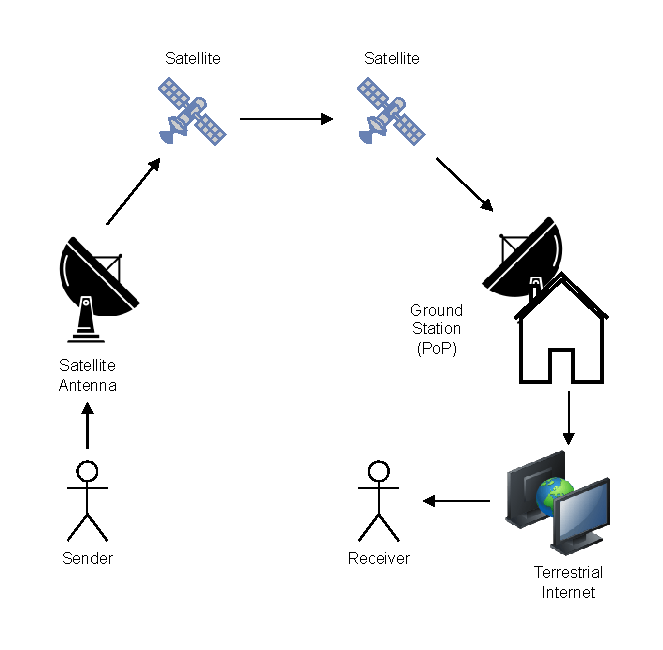
\includegraphics[width=\textwidth]{./chapters/background/img/satcom-structure.drawio.pdf}
	\caption{The structure of satellite communication.}
	\label{fig:sat-com-explained}
\end{figure}

The structure is illustrated in Figure~\ref{fig:sat-com-explained}.
Initially, there is a sender connected to a satellite antenna provided by the specific networked satellite ISP.
The satellite antenna is also colloquially called "dishy".
From the senders' perspective, there is no different use compared to a traditional terrestrial internet connection.
The antenna will send packets to a satellite that might either forward the packets to another satellite or directly send them
to a nearby \ac{GS} (also called \ac{PoP}). The \ac{GS} serves as an "entry point" to the terrestrial internet.
A \ac{GS} can forward packets through wired connections, so they will reach the receiver eventually.

The technology of communicating with satellites will not be explained here.
Amongst others, it is described by Pratt~et~al. \cite{pratt2019satellite}.

Theoretically, the propagation of data in satellite communication happens at the speed of light.
However, the latencies still vary a lot depending on the choice of networked satellite ISP.
Each of them provides a different satellite constellation. One of the dominating factors is the
altitude of the constellation. The higher the satellites are positioned, the more region a single satellite covers.
Therefore, fewer satellites are required to cover a specific region, which reduces costs.

Overall, one differentiates between \ac{GEO} (35'786 km altitude), \ac{MEO} (2'000 - 35'786 km altitude), and \ac{LEO} (< 2'000 km altitude) satellite constellations.
One can see that this has a significant impact on the latency.

\begin{equation}
	\frac{2 \cdot 35'786 km}{300'000 \frac{km}{s}} \approx 0.240 s
	\label{eq:geo-min-latency}
\end{equation}
\begin{equation}
	\frac{2 \cdot 550 km}{300'000 \frac{km}{s}} \approx 0.004 s
	\label{eq:starlink-min-latency}
\end{equation}

A \ac{GEO} constellation has a minimum latency of around 240 ms, as shown in Equation~\ref{eq:geo-min-latency}, assuming a packet needs to reach a satellite in GEO altitude and get back to the earth's surface.
On the other hand, Equation~\ref{eq:starlink-min-latency} shows that a \ac{LEO} satellite constellation at an altitude of 550 km (like in the case of Starlink) has a minimum latency of only 4 ms.
Research has shown that even in practice \ac{LEO} constellations are superior compared to \ac{GEO} constellations, especially in terms of latency \cite{DBLP:journals/pacmnet/RamanVCSZ23, Segan2020}.
However, terrestrial internet performed better compared to \ac{LEO} constellations \cite{DBLP:conf/www/MohanFCBRMO24, DBLP:conf/infocom/MaCZCML23}.

\subsection{Bent-Pipes} \label{sec:bent-pipes}

Ground stations are required for satellites to route packets to a receiver. Depending on the location of the sender, the first satellite on the route might have to forward packets to a different satellite (using an \ac{ISL}) in order to reach a region with a \ac{GS}. Such a route is called "Bent-Pipe". Depending on the number of satellites on the route, it is called an "n-hop-bent-pipe". If there is only a single satellite involved, it is a 1-hop-bent-pipe.

% TODO: Find more sources pro and con
It is in question how the bent-pipe influences the performance and behavior of a networked satellite system. Research still discusses whether bent-pipes provide a positive (\cite{Hauri2020}) or negative (\cite{DBLP:conf/www/MohanFCBRMO24}) impact.

